\chapter{Planung}

Ein essentieller schritt in der Softwareentwicklung ist die Planung. Auch für dieses Projekt habe ich mich ausführlich mit der Planung auseinander gesetzt. Erste habe ich mir ein generelles Konzept erarbeitet, folgend diese Ideen spezifiziert und anschließend in anschaulichen visualisiert.

\section{Entity-Relation-Diagramm}
Zu Beginn erstellte ich das Entity-Relation-Diagramm, weil dort die Beziehungen zwischen Entitätstypen genauer beschrieben werden. 

\begin{figure}[h]
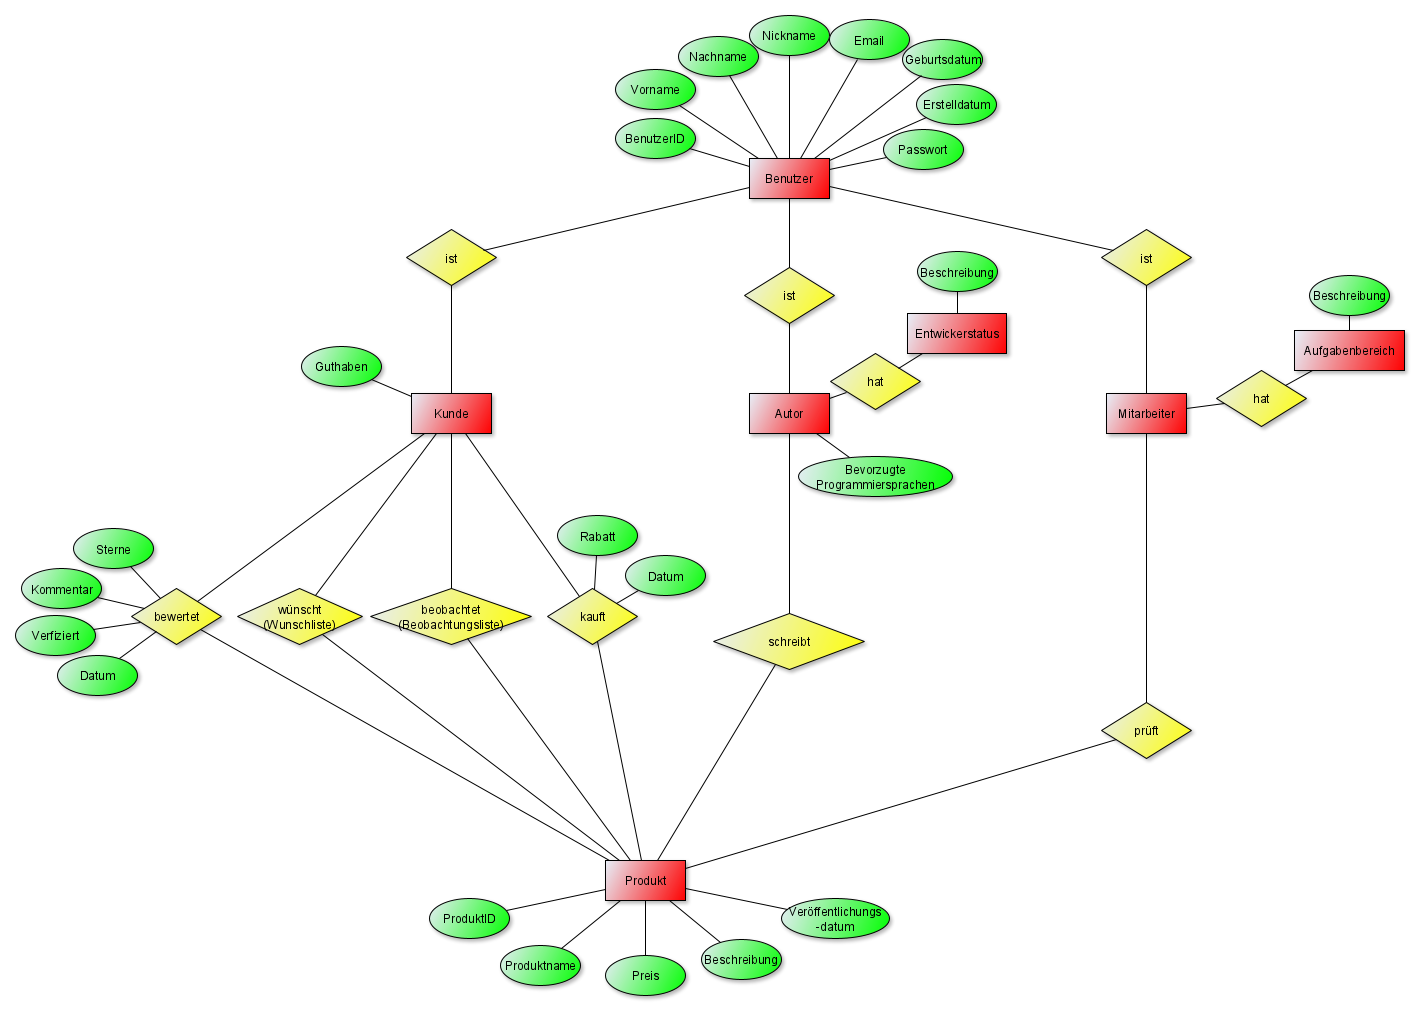
\includegraphics[width=1\textwidth]{D:/Schule/SWR/Verkaufsprojekt/master/Planning/ER-Diagram v1.png}
\caption{Entity-Relation-Diagramm}
\end{figure}

\newpage
\section{UML-Klassen-Diagramm}

Nachdem ich das erste ER-Diagramm hatte, erstellte ich ein UML-Klassen-Diagramm, wo man eine Übersicht darüber bekommt, welche Klassen und Datentypen notwendig sind. Zu bemerken ist, dass die Inhalte der Enumerationen stetig geändert werden.

\begin{figure}[h]
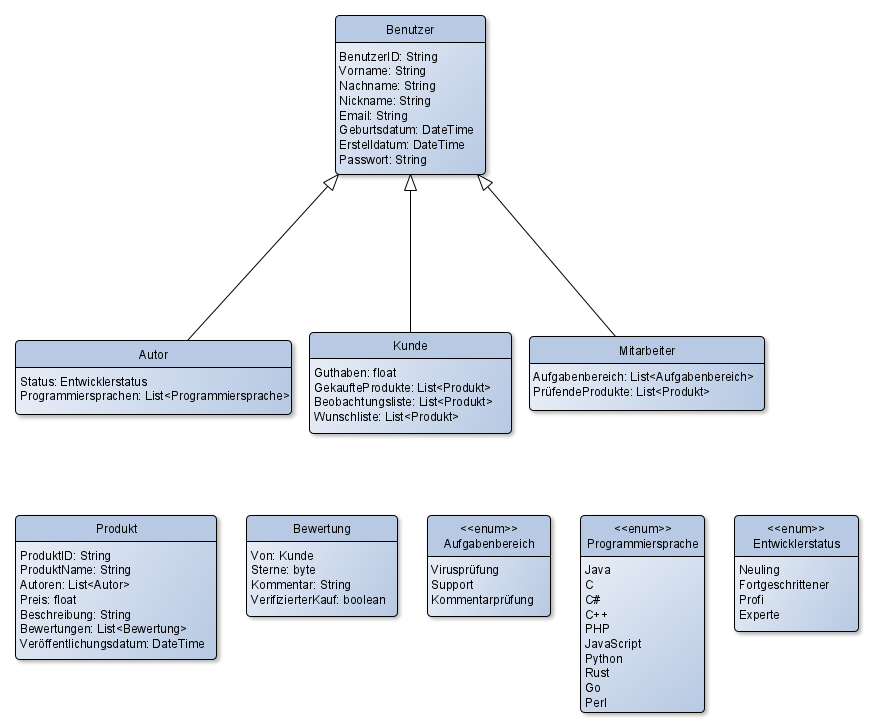
\includegraphics[width=1\textwidth]{D:/Schule/SWR/Verkaufsprojekt/master/Planning/UML-Diagram v1.png}
\caption{UML-Klassen-Diagramm}
\end{figure}

\newpage
\section{Programmablaufplan}

Für einen übersichtlichen Überblick der Funktionen der Applikation ist ein Programmablaufplan sinnvoll. Vor allem zum Testen der Applikation ist er gut geeignet, da man alle möglichen Zweige einzeln testen kann.\\
\\Der Programmablaufplan befindet sich auf GitHub: \url{https://github.com/OliverSchlueter/Verkaufsprojekt/tree/master/Planning}

\begin{figure}[h]
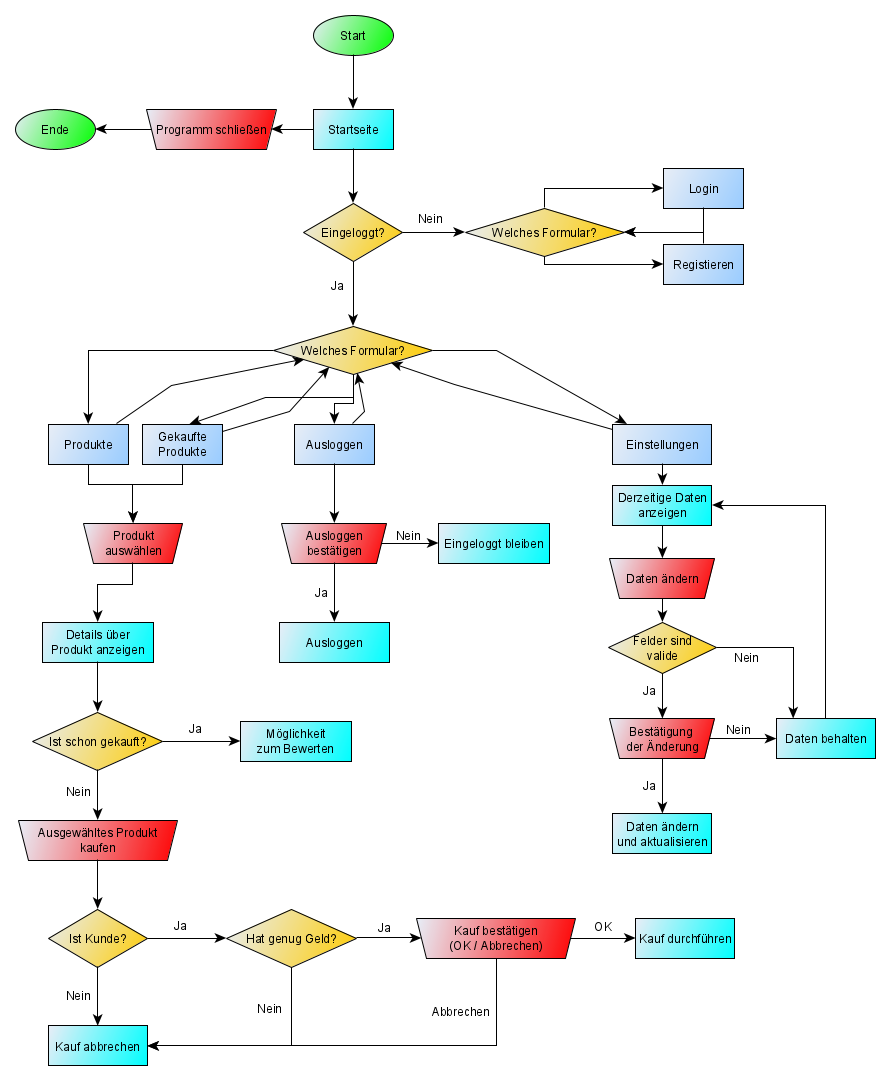
\includegraphics[width=1\textwidth]{D:/Schule/SWR/Verkaufsprojekt/master/Planning/PAP v1.png}
\caption{Programmablaufplan}
\end{figure}

\newpage
\section{Datenbank Skript}
Relativ schnell nach dem Erstellen der Diagramme, schrieb ich das Skript zur Erzeugung der Datenbank, wobei vorher die Überlegung der Wahl des DBMS zu treffen war. In meinen Projekt benutze ich eine MySQL-Datenbank für die Speicherung der Benutzer- sowie Produktdaten, um auf diese zuzugreifen ist diese mit einer lokalen Microsoft Access-Datenbank synchronisiert.\\
Das Skript finden sie hier: \url{https://github.com/OliverSchlueter/Verkaufsprojekt/blob/master/Planning/DB-Script.sql}